\documentclass[]{article}
\usepackage[german]{babel}
\usepackage{graphicx}
\usepackage{tabularx}
\usepackage[backend=bibtex, natbib=true]{biblatex}
\usepackage{listings}
\usepackage{tikz}

\lstset{%
	basicstyle=\ttfamily\scriptsize,        % Code font, Examples: \footnotesize, \ttfamily
	keywordstyle=\color{blue!80!black},     % Keywords font ('*' = uppercase)
	commentstyle=\color{gray},              % Comments font
	numbers=left,                           % Line nums position
	numberstyle=\tiny,                      % Line-numbers fonts
	stepnumber=1,                           % Step between two line-numbers
	numbersep=5pt,                          % How far are line-numbers from code
	backgroundcolor=\color{gray!10!white},  % Choose background color
	frame=none,                             % A frame around the code
	tabsize=2,                              % Default tab size
	captionpos=b,                           % Caption-position = bottom
	breaklines=true,                        % Automatic line breaking?
	breakatwhitespace=false,                % Automatic breaks only at whitespace?
	showspaces=false,                       % Dont make spaces visible
	showstringspaces=false                  %
	showtabs=false,                         % Dont make tabls visible
	columns=flexible,                       % Column format
	morekeywords={},                        % Specific keywords
	stringstyle=\color{green!50!black},%
}%

\bibliography{bibliography}
%opening
%Here you can enter your names and titleof your report
\title{Weekly Reports}
\author{Luftqualität in Innenräumen - Gruppe 1}

\begin{document}

\maketitle

\begin{table}[h!]
	\centering
	\begin{tabular}{|c|c|c|}
		\hline
		{\textbf{Name}}				&		{\textbf{Matrikel Nr.}} & {\textbf{Arbeitsaufwand (h)}} \\
		\hline
		Friedrich Just				&		1326699 				&	17,00	\\
		\hline
		Stipe Knez				&		1269206 				&	17,00	\\
		\hline
		Lucas Merkert				&		1326709					&	17,00	\\
		\hline
		Achim Glaesmann				&		1309221					&	19,00	\\
		\hline
		Max-Rene Konieczka			&		1211092					&	16,00	\\
		\hline
		Can Cihan Nazlier			&		1179244					&	21,00	\\
		\hline
	\end{tabular}
	\caption{Arbeitsaufwand dieser Woche}
	\label{tab:worakload}
\end{table}



\section{Überblick}


\subsection{Friedrich Just}
In dieser Woche habe ich mich mit dem Pflichtenheft befasst, mir angesehen, welche Sensoren wir haben und was diese können. Ich habe mir die passenden Datenblätter~\cite{datasheetcss811}~\cite{datasheetscd41}~\cite{datasheetsht21} zusammengesucht. In diesen sind mir einige Begriffe unklar gewesen, wie VOC bzw. TVOC~\cite{tvoc}, eCO2~\cite{eco2} und relative Luftfeuchtigkeit~\cite{realtiveluftfeuchtigkeit}. Dazu habe ich recherchiert. Danach habe ich diese durchgearbeitet, um die Sensoren und deren Funktionsweise genauer zu verstehen. Außerdem habe ich mich mit den Funkmodulen auseinandergesetzt und wollte den Temperatursensor aus dem ZigBee-Set(LM73) und das ZigBee-Netzwerk miteinander verbinden, so dass die Sensordaten an den Koordinator weitergeleitet werden. Während dieser Zeit habe ich mich erneut mit dem I$^2$C-Bus und der Übertragung von Daten beschäftigt.
{Abbildung \ref{img:scd41_commandset}}
i2c Adresse 0x62 ~\cite{datasheetscd41}Seite 7

\begin{figure}[!h]
	\centering
	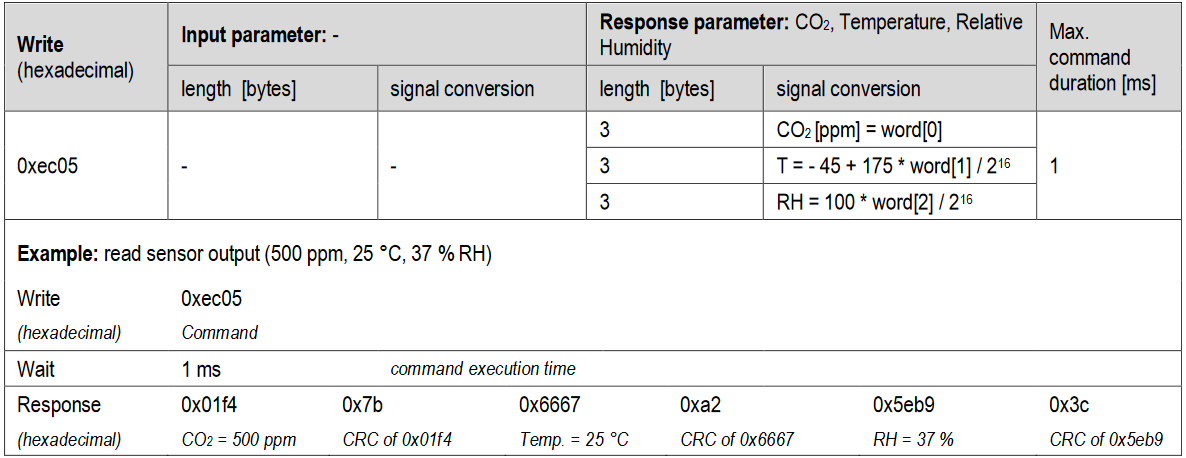
\includegraphics[scale=0.40]{images/scd41_umrechnung}
	\caption{Auswertung einer Messung ~\cite{datasheetscd41}}
	\label{img:scd41_umrechnung}
\end{figure}
\begin{figure}[!h]
	\centering
	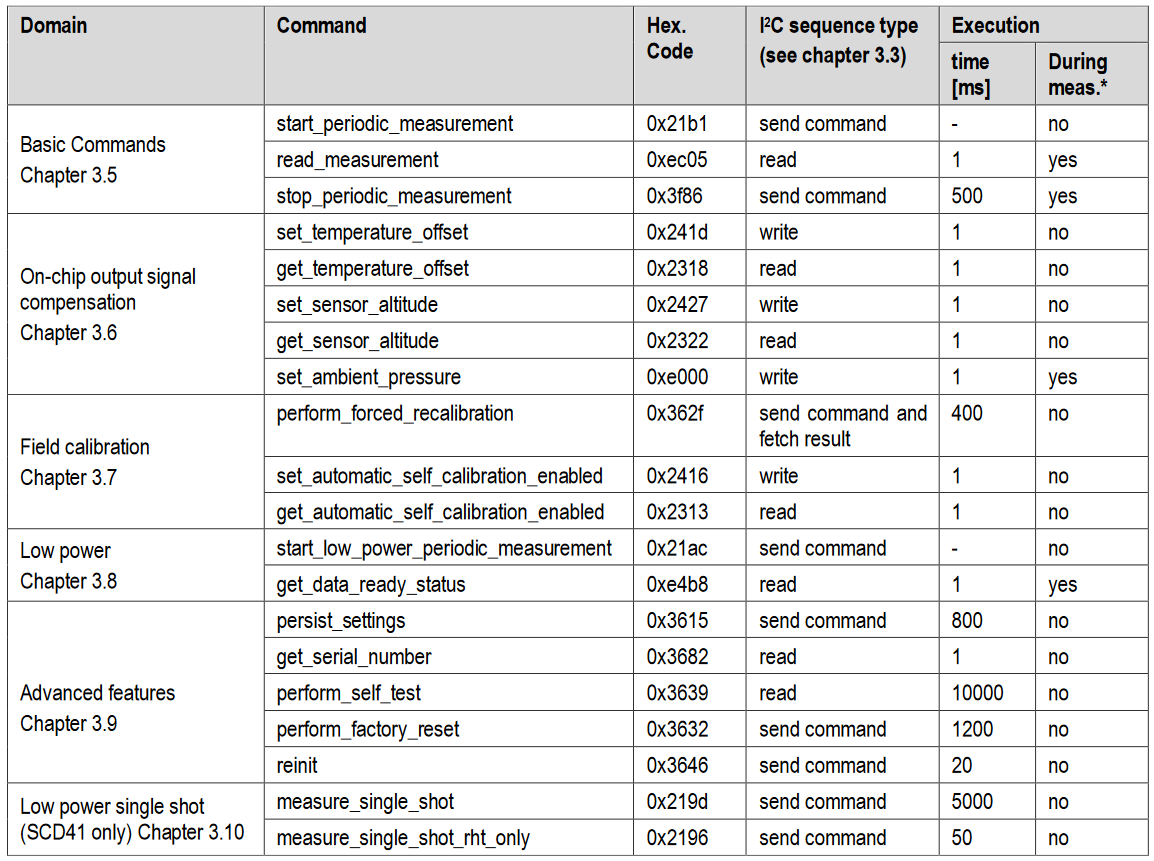
\includegraphics[scale=0.40]{images/scd41_commandset}
	\caption{Befehle zum Ansteuern des SCD41 Sensors~\cite{datasheetsht21}}
	\label{img:scd41_commandset}
\end{figure}


\subsection{Stipe Knez}
In der ersten  Woche lag der Fokus auf zwei Bereichen: Dem Nachbessern des Pflichtenhefts nach einer internen Besprechnung und dem Schaffen einer geeigneten Programmierumgebung für den weiteren Verlauf des Projektes auf meinem Rechner samt der Einarbeitung in Javascript.
Neben dem ausbessern vorhandenem Inhalts haben wir uns Gedanken über unsere Vorgehensweise gemacht woraufhin ich nach Vorgehensweisen recherchiert habe~\cite{scrum}, von denen wir uns für unser eigenes Projekt inspirieren lassen können. Anschließend habe ich unsere Vorgehensweise nach kurzer Absprache und Beratung mit der Gruppe ausformuliert und für das Pflichtenheft vorbereitet.

Des Weiteren spielte wie zuvor erwähnt auch das Schaffen einer geeigneten Programmierumgebung samt der Einarbeitung in Javascript diese Woche für mich eine große Rolle. Zuerst habe ich die beiden IDEs Webstorm und IntelliJ IDEA Ultimate eingerichtet. Dabei soll Webstorm der Entwicklung in Javascript und IntelliJ der Entwicklung in Java dienen. Weil ich in Javascript noch nicht allzu viel Programmiererfahrung gesammelt habe, habe ich mich in die Sprache eingearbeitet. Hilfreich waren dabei eine Javascript Dokumentation~\cite{JS_docu} sowie Lerninhalte in Videoform~\cite{javascript_tut}. Außerdem habe ich noch die GitHub Desktop Anwendung auf meinem Rechner eingerichtet und mich mit LaTex auseinandergesetzt und die dazugehörigen Anwendungen installiert.

\subsection{Lucas Merkert}
Einarbeitung SHT21: Der SHT21 Sensor wird über den I2C-Bus angesprochen {Abbildung \ref{img:sht21_commandset}} um die Temperatur und relative Luftfeuchtigkeit zu messen. Der Sensor gibt die Temperatur in einer 14 Bit Auflösung und die Relative Luftfeuchtigkeit in einer 12 Bit Auflösung zurück. Die Werte können dann mit den Formel aus {Abbildung \ref{img:sht21_tempformula}} und {Abbildung \ref{img:sht21_rhformula}} berechnet werden. Dabei ist das Problem aufgetreten wie genau man den Sensor über HAL\_WriteI2cPacket() anspricht.
\begin{figure}[h]
	\centering
	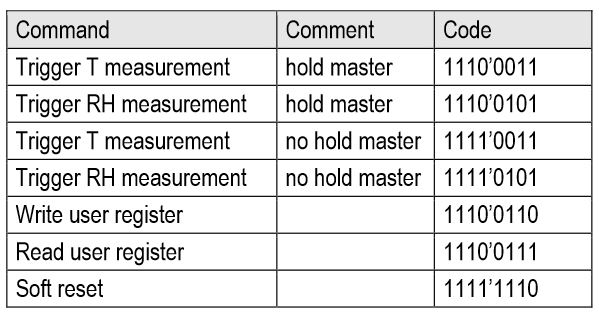
\includegraphics[scale=0.60]{images/sht21_commandset}
	\caption{Befehle zum Ansteuern des SGT21 Sensors, T für Temperatur, RH für relative Luftfeuchtigkeit~\cite{datasheetsht21}}
	\label{img:sht21_commandset}
\end{figure}
\begin{figure}[h]
	\centering
	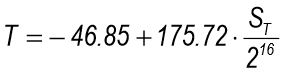
\includegraphics[scale=0.60]{images/sht21_tempformula}
	\caption{Formel zur Berechnung der Temperatur~\cite{datasheetsht21}}
	\label{img:sht21_tempformula}
\end{figure}
\begin{figure}[h]
	\centering
	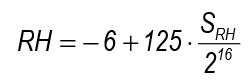
\includegraphics[scale=0.60]{images/sht21_rhformula}
	\caption{Formel zur Berechnung der relativen Luftfeuchtigkeit~\cite{datasheetsht21}}
	\label{img:sht21_rhformula}
\end{figure}

\subsection{Achim Glaesmann}
In der vergangenen Woche wurden von mir folgende Aufgaben bearbeitet. Zunächst wurde das Pflichtenheft ausgebessert, wobei von mir die Projektbeschreibung angefertigt wurde.
Außerdem war es nötig die für die Entwicklung vorraussichtlich benötigte Software zu installieren. 
Dazu zählte die Installation von Github, so wie eine entsprechende Einarbeitung. Die Installation von Intellij IDEA als IDE für die Java Entwicklung sowie eine entsprechende Einarbeitung.
Die Installation von WebStorm als IDE für die Javascript Entwicklung so wie eine entsprechende Einarbeitung. Die Installation von MikTex als Compiler für Tex files so wie eine entsprechende 
Einarbeitung in die Syntax von LaTex. Weiterhin wurde sich in einer kleinen Gruppe Mittwochs getroffen um die Sensoren in Verbindung mit den Mikrokontrollern zu testen. Bis 
jetzt war es uns nicht möglich die Daten auszulesen, es ist beabsichtigt das Problem in der kommenden Woche zu lösen. Eine ausgiebige Recherche der Datenblätter sollte hierbei
helfen.~\cite{datasheetsht21}q Es wurden weiterhin Recherchen betrieben zur Risikoabschätzung der Aerosolbelastung basierend auf dem CO2 gehalt der Umgebungsluft. Hierbei wurden mehrere Paper gelesen wobei 
eines bis jetzt die vielversprechensten Informationen lieferte. ~\cite{co2letter} Die Recherche wird in den kommenden Wochen fortgeführt. Weiterhin wurde die Präsentation zu Analog Digital Wandlern 
angefertigt. Das Übungsblatt 2 wurde korrigiert. Es wurden insgesamt 4 Meetings mit der Gruppe gehalten.

\subsection{Max-Rene Konieczka}
Aufbauend zur letzten Woche, hat man sich mit der korrekten Einrichtung des Projektes beschäftigt, welches von Can Cihan Nazlier letzte Woche konfiguriert wurde. Darüber hinaus wurde influxDB installiert, was sich gut dafür eignet Zeitreihen-Daten zu verwalten. Da die Applikation eine Reactive Web App sein wird, wurden Recherchen zum Thema Websockets und SocketIO gemacht. SocketIO ist eine JavaScript-Bibliothek, welche für Echtzeit-Webanwendungen verwendet wird. Diese ermöglicht bidirektionale Echtzeit-Kommunikation zwischen dem Browser und einem Server. Dadurch werden Benutzereingaben schneller behandelt und die App läuft flüssiger. Websocket wiederum ist ein Netzwerkprotokoll, was auf TCP basiert. SocketIO macht sich das Websocketprotokoll zunutze.

\subsection{Can Cihan Nazlier}
Im Verlauf der Woche habe ich unserer Projekt konfiguriert und auf Github gepusht. Er besteht aus einem backend, frontend, models und einem electron Teil. Ich habe das frontend mit node so konfiguriert, dass es sich in den electron Ordner buildet und wir eine desktop application daraus erstellen können. Das backend habe ich mit express aufgesetzt und die von Herrn Merkl empfohlene Datenbank influxDB integriert. Zudem habe ich angefangen das Zeichentool zu programmieren und einen ersten Prototypen zu entwickeln. Des weiteren habe ich mich mit den Schnittstellen befasst und dem Datenaustausch zwischen den modulen und den Mockup. Ich habe erste Datentransfermodelle entwickelt und im Laufe der Woche werde ich Mockup Daten erstellen und mit diesen erste use-cases nachstellen. Ich habe mich auch noch mit Socket IO auseinandergesetzt, weil wir mit Websockets arbeiten werden, um eine reactive app zu gestalten.

\printbibliography
%----------------------------------------------------------------------------
% Bibliography
%----------------------------------------------------------------------------	

\end{document}
